% =====================================================================
%  Plan4ARI -- D4.1 (A4 revision)
%  Updated scientific plan for local and global autonomous motion planning
%  Draft of D4.1 Sections 2 (scenario/requirements), 8 (revised architecture),
%  9 (selected methods and fallbacks) and 10 (benchmarking, Task 4.7)
%
%  Bibliography: shared with the SOTA knowledge base (../SOTA/latex/references.bib)
%  Build: latexmk -pdf plan_update.tex
% =====================================================================
\documentclass[10pt,a4paper]{article}
\usepackage[utf8]{inputenc}
\usepackage[T1]{fontenc}
\usepackage{lmodern}
\usepackage[a4paper,margin=2.1cm]{geometry}
\usepackage{amsmath,amssymb}
\usepackage{booktabs,tabularx,longtable,multirow}
\usepackage[dvipsnames,table]{xcolor}
\usepackage{tikz}
\usetikzlibrary{arrows.meta,positioning,fit,backgrounds,calc}
\usepackage{enumitem}
\usepackage{cite}
\usepackage{microtype}
\usepackage[colorlinks=true,linkcolor=MidnightBlue,citecolor=MidnightBlue,urlcolor=MidnightBlue]{hyperref}
\setlist{itemsep=1pt,topsep=3pt,leftmargin=*}
\newcolumntype{L}[1]{>{\raggedright\arraybackslash}p{#1}}
\newcolumntype{Y}{>{\raggedright\arraybackslash}X}

\title{\textbf{Plan4ARI -- Activity 4: Updated Scientific Plan for Local and Global Autonomous Motion Planning}\\[4pt]
\large Draft contribution to D4.1 (A4 revision): scenario, revised architecture, selected methods, benchmarking plan}
\author{CNR-STIIMA, Industrial Robotics Lab}
\date{October 2026 -- Draft v0.1 -- for consortium discussion}

\begin{document}
\maketitle

\begin{abstract}
\noindent
Since the submission of Plan4ARI, sampling-based motion planning and sampling-based model predictive control have changed substantially: planners now answer collision-free queries in microseconds on a CPU~\cite{thomason2024vamp}, and Model Predictive Path Integral (MPPI) control has become a practical, derivative-free receding-horizon method for manipulators and mobile robots~\cite{williams2018tro,bhardwaj2021storm,macenski2023nav2survey}. This note updates the scientific plan of Activity~4 accordingly. The original pillars --- informed sampling-based planning with multi-path reuse (T4.2) and MPC micro-interpolation in the Core IPC (T4.3) --- are \emph{retained}; an MPPI-based \emph{look-ahead} layer is \emph{added} between them to explore the task redundancy ahead of the robot, handle discrete configuration alternatives and react to scene changes. We make explicit the end-to-end pipeline, starting from the optimal localisation of the robot with respect to the task, map every block onto the Open IPC / Core IPC architecture, require the framework to be robot-agnostic, and define the application set and benchmarking protocol of Task~4.7, where welding of large structures is validated on real hardware and all other applications in simulation.
\end{abstract}

% ---------------------------------------------------------------------
\section{What changes with respect to the proposal}
% ---------------------------------------------------------------------
\begin{table}[h]
\centering\small
\caption{Original plan (Project Description, \S A.4 and \S E.3) versus updated plan.}\label{tab:delta}
\begin{tabularx}{\textwidth}{@{}L{3.1cm}YY@{}}
\toprule
 & \textbf{Original plan} & \textbf{Updated plan} \\
\midrule
Global / online planning (T4.2) & Informed sampling-based planner, mixed global/local sampling, multi-path reuse & \textbf{Retained}. Also used for transfer motions (retract, reconfigure, approach) and for station-level feasibility; vectorised CPU primitives~\cite{thomason2024vamp} adopted for speed \\
Local reactive layer & MPC ``alongside'' the sampling-based planner & \textbf{New: MPPI look-ahead} over the task null space, with multiple goals (configuration alternatives), guided by the sampling-based planner~\cite{trevisan2024biasedmppi,tao2023rrtmppi} \\
Micro-interpolation (T4.3) & MPC in the Core IPC, speed override, visual servoing & \textbf{Retained}, specified as path--velocity layer with hard joint limits and a speed band~\cite{faulwasser2017pathfollowing,lange2016pathaccurate,faroni2020scaling} \\
Task localisation & Implicit (industrial practice) & \textbf{Explicit pipeline stage}: optimal placement of robot / AGV / external axis with respect to the segmented task~\cite{weingartshofer2021tcpbase,nguyen2023taskclustering} \\
Safety-aware cost & ISO/TS 15066 cost in the replanner~\cite{faroni2022safetyaware} & \textbf{Retained}, evaluated per rollout in MPPI and per edge in the sampling-based planner \\
Robot dependence & COMAU platform & \textbf{Robot-agnostic}: kinematic abstraction for any serial arm, external axes and mobile base \\
Benchmarking (T4.7) & $\geq$50 scenarios, OMPL baseline, GPU planners not compared & Same KPIs; \textbf{application catalogue} (Sect.~\ref{sec:bench}); welding on hardware, others in simulation; GPU methods in a separate track \\
\bottomrule
\end{tabularx}
\end{table}

% ---------------------------------------------------------------------
\section{Reference application and requirements}\label{sec:app}
% ---------------------------------------------------------------------
\paragraph{Reference application.} Arc welding of very large metal structures by an industrial arm mounted on an AGV (optionally on an interpolated linear axis). The AGV is placed at a station and the arm welds a portion of the structure; base motion interpolated with the arm during welding is a secondary, theoretically relevant option. The task is \emph{under-constrained}: the seam point must be reached exactly, the torch axis may lie within a cone of about $10^\circ$ around the nominal direction (possibly anisotropic between work and travel angle), the rotation about the torch axis is almost always free, and the travel speed must stay constant within $\pm10\%$ along the whole seam. Because of the size of the structure the arm may have to change configuration: stop, retract, reconfigure, approach and restart about 1\,cm before the detach point.

\paragraph{Requirements derived for the framework.}
\begin{enumerate}[label=R\arabic*.]
\item \textbf{Exact task, free redundancy.} Task constraints (position, axis) are hard; tolerances (cone, roll, external axes, base) are exploited as optimisation freedom~\cite{demaeyer2017descartes,chen2025cooptimization}.
\item \textbf{Speed band.} Travel speed within a fixed band ($\pm10\%$) under joint velocity, acceleration and jerk limits~\cite{lange2016pathaccurate}.
\item \textbf{Planned reconfigurations.} Fewest stop--reconfigure--restart cycles, with planned transfer motions and restart overlap~\cite{yin2024dpbreakpoints,wang2025anytimetracking}.
\item \textbf{Optimal task localisation.} Station / base / rail placement chosen so that whole task segments are feasible~\cite{weingartshofer2021tcpbase,wachter2024tcpbase}.
\item \textbf{Registration.} Mobile platforms on large workpieces show centimetre-level errors without local registration~\cite{zhao2021mobilemachining}: the plan is executed on the locally registered task (seam scan~\cite{wang2026torchposture}, Activity~3).
\item \textbf{Human-shared space.} ISO/TS 15066-aware costs and certified speed adaptation~\cite{faroni2022safetyaware,gursoy2026cosmik}.
\item \textbf{Robot-agnostic.} Any serial arm (non-cuspidal or cuspidal~\cite{elias2025cuspidal}), joints with range beyond $\pm\pi$, external linear/rotary axes, mobile bases.
\item \textbf{Industrial integration.} Deterministic, repeatable outputs; dockerised actions in MI.RA/Dexter; hard real-time Core IPC.
\end{enumerate}

% ---------------------------------------------------------------------
\section{Updated approach: sampling-based planning \emph{and} MPPI}
% ---------------------------------------------------------------------
Industrial controllers rely on \emph{look-ahead}: a buffer of future path samples is analysed to adapt speed under kinematic limits~\cite{lange2016pathaccurate}. For under-constrained tasks this look-ahead is limited to a single, pre-computed joint solution. MPPI can be seen as a \emph{stochastic look-ahead} that explores the redundancy ahead of the robot: it samples many short futures of the null-space variables (torch roll, cone tilt, external axis), evaluates them with arbitrary, non-smooth costs (collisions with the structure, joint-limit and singularity margins, ISO/TS 15066 slowdown, speed feasibility) and returns an improved plan every cycle~\cite{williams2018tro}. Recent work shows null-space sampling with exact task satisfaction~\cite{wang2024constrainedpi,lee2026prmppi}, its deterministic counterpart~\cite{sun2024nullspacempc}, and planners that guide MPPI~\cite{tao2023rrtmppi,trevisan2024biasedmppi}.

Sampling-based planning remains essential where MPPI is weak: long transfer motions in clutter (local minima), station-level feasibility and multi-path reuse. The two are complementary: \emph{the sampling-based planner proposes, MPPI refines and reacts, the Core-IPC MPC certifies}.

\paragraph{Multi-goal MPPI look-ahead.} The goal of the look-ahead is a Cartesian task segment (e.g.\ ${\sim}10$\,cm of seam) together with a \emph{set of start configurations}, one per inverse-kinematics solution class (up to 8 for a non-cuspidal 6R arm, up to 16 for cuspidal arms, multiplied by joint turns where ranges exceed $\pm\pi$~\cite{elias2025cuspidal}). For each class MPPI optimises the null-space variables along the segment with exact IK on that class. Classes are \emph{selected, never blended}~\cite{liu2026clusteringmppi,wang2026mppiem}. Continuing on the current class has no transfer cost; switching class costs a transfer (planned by the sampling-based planner, first to the nominal start for a cost estimate, then to the optimised start for the actual connection, with a consistency check) plus the restart overlap. A time-dilation factor $\lambda=\max_j |\dot q_j^{\mathrm{req}}|/\dot q_j^{\max}$ along each rollout measures speed feasibility ($\lambda\le 1/0.9$ for a $\pm10\%$ band), so that a reconfiguration emerges from cost comparison when the current class cannot keep the speed or approaches joint limits. The full design review, with 24 identified risks and their status, is kept in the project knowledge base.

% ---------------------------------------------------------------------
\section{End-to-end pipeline}\label{sec:pipeline}
% ---------------------------------------------------------------------
\begin{figure}[t]
\centering
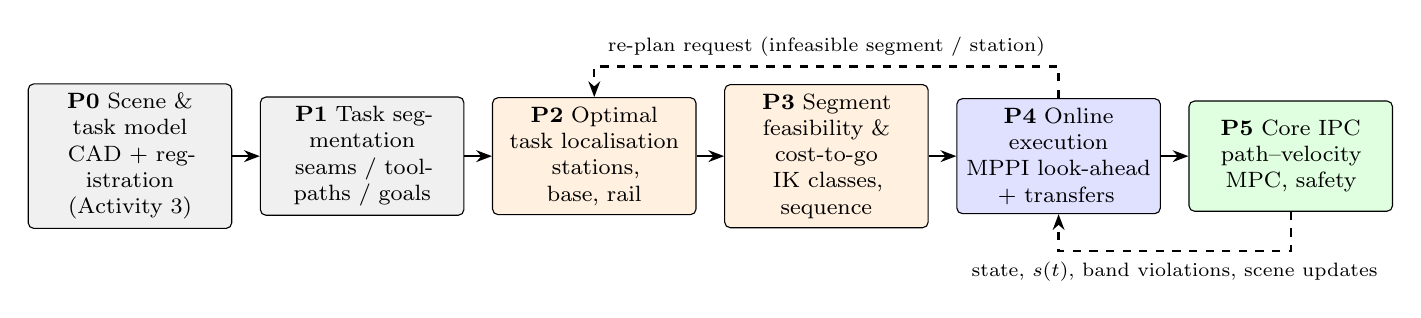
\begin{tikzpicture}[font=\footnotesize, node distance=3.5mm,
  st/.style={draw,rounded corners=2pt,align=center,text width=2.35cm,minimum height=14mm,fill=#1!12},
  arr/.style={-{Stealth[length=2mm]},thick}]
\node[st=gray] (p0) {\textbf{P0} Scene \& task model\\CAD + registration\\(Activity 3)};
\node[st=gray, right=of p0] (p1) {\textbf{P1} Task segmentation\\seams / toolpaths / goals};
\node[st=orange, right=of p1] (p2) {\textbf{P2} Optimal task localisation\\stations, base, rail};
\node[st=orange, right=of p2] (p3) {\textbf{P3} Segment feasibility \& cost-to-go\\IK classes, sequence};
\node[st=blue, right=of p3] (p4) {\textbf{P4} Online execution\\MPPI look-ahead + transfers};
\node[st=green, right=of p4] (p5) {\textbf{P5} Core IPC\\path--velocity MPC, safety};
\foreach \a/\b in {p0/p1,p1/p2,p2/p3,p3/p4,p4/p5} \draw[arr] (\a) -- (\b);
\draw[arr,dashed] (p5.south) -- ++(0,-5mm) -| node[pos=0.25,below]{\scriptsize state, $s(t)$, band violations, scene updates} (p4.south);
\draw[arr,dashed] (p4.north) -- ++(0,4mm) -| node[pos=0.25,above]{\scriptsize re-plan request (infeasible segment / station)} (p2.north);
\end{tikzpicture}
\caption{End-to-end pipeline. Orange: planning before execution (Open IPC, seconds to minutes). Blue: online planning (Open IPC, 10--100\,Hz). Green: hard real time (Core IPC, 1\,kHz).}\label{fig:pipeline}
\end{figure}

\begin{description}[leftmargin=0pt]
\item[P0 -- Scene and task model.] CAD of the workpiece and cell, registered with the sensing modules of Activity~3; local registration at each station (R5).
\item[P1 -- Task segmentation.] The task is split into segments with homogeneous constraints (for welding: seams split at corners, interruptions and process changes; corners at constant speed are where joint-speed limits break~\cite{gautier2024weldingbase}).
\item[P2 -- Optimal task localisation.] Selection of the minimum set of stations (AGV poses, rail intervals, or the fixed base of an arm) such that each segment is \emph{path-wise feasible} from at least one station: set-cover over segments~\cite{nguyen2023taskclustering} with a continuous-branch test~\cite{weingartshofer2021tcpbase}, the speed-feasibility check $\lambda$, margins for positioning error and orientation tolerances; candidates from inverse reachability maps~\cite{makhal2018reuleaux} and joint base--path optimisation~\cite{zhao2025bstar}. This stage was implicit in the proposal and is made explicit here.
\item[P3 -- Segment feasibility and cost-to-go.] For each station and segment: feasible IK classes, nominal null-space seeds, reconfiguration points and a cost-to-go table, computed by a deterministic layered-graph / dynamic-programming planner~\cite{yin2024dpbreakpoints,demaeyer2017descartes}; also the sequence of segments and transfers (with Activity 2 for multi-robot allocation~\cite{tang2023dualrobotweld}).
\item[P4 -- Online execution.] Multi-goal MPPI look-ahead on the registered segment (R1--R3), with the cost-to-go from P3 as terminal cost; transfer motions by the sampling-based planner of T4.2; reaction to scene changes and humans.
\item[P5 -- Core IPC.] Path--velocity layer: the joint path $q(s)$ from P4 is time-parametrised within the speed band under hard limits; speed override and safety rules (ISO/TS 15066); synchronous sensor input (seam tracking, visual servoing). A band violation is reported upstream as a detach request, never resolved by an unplanned stop during the process.
\end{description}

% ---------------------------------------------------------------------
\section{Open IPC / Core IPC architecture}\label{sec:arch}
% ---------------------------------------------------------------------
\begin{figure}[t]
\centering
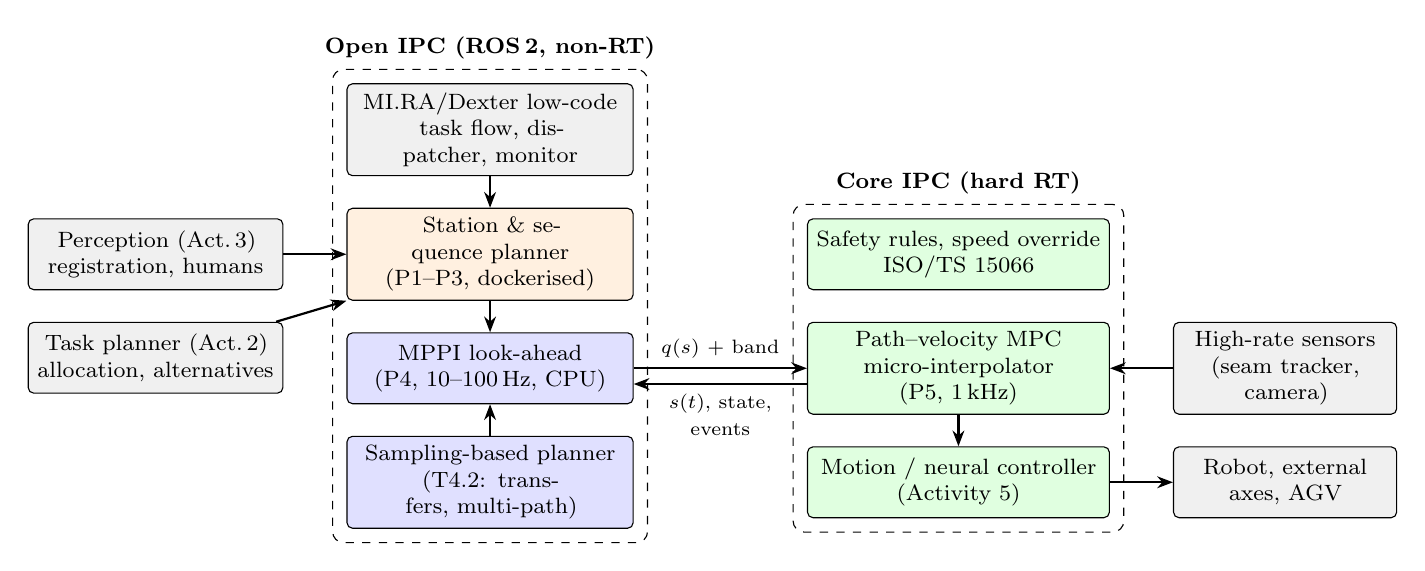
\begin{tikzpicture}[font=\footnotesize,
  blk/.style={draw,rounded corners=2pt,align=center,fill=#1!12,minimum height=9mm},
  arr/.style={-{Stealth[length=2mm]},thick},
  zone/.style={draw,dashed,rounded corners=4pt,inner sep=5pt}]
% Open IPC
\node[blk=gray,text width=3.4cm] (dex) at (0,0) {MI.RA/Dexter low-code\\task flow, dispatcher, monitor};
\node[blk=orange,text width=3.4cm,below=4mm of dex] (sta) {Station \& sequence planner\\(P1--P3, dockerised)};
\node[blk=blue,text width=3.4cm,below=4mm of sta] (mppi) {MPPI look-ahead\\(P4, 10--100\,Hz, CPU)};
\node[blk=blue,text width=3.4cm,below=4mm of mppi] (sbp) {Sampling-based planner\\(T4.2: transfers, multi-path)};
\node[blk=gray,text width=3.0cm,left=8mm of sta] (perc) {Perception (Act.\,3)\\registration, humans};
\node[blk=gray,text width=3.0cm,below=4mm of perc] (task) {Task planner (Act.\,2)\\allocation, alternatives};
\node[zone,fit=(dex)(sta)(mppi)(sbp),label={[font=\footnotesize\bfseries]above:Open IPC (ROS\,2, non-RT)}] (open) {};
% Core IPC
\node[blk=green,text width=3.6cm,right=22mm of mppi] (mpc) {Path--velocity MPC\\micro-interpolator (P5, 1\,kHz)};
\node[blk=green,text width=3.6cm,above=4mm of mpc] (saf) {Safety rules, speed override\\ISO/TS 15066};
\node[blk=green,text width=3.6cm,below=4mm of mpc] (ctl) {Motion / neural controller\\(Activity 5)};
\node[zone,fit=(saf)(mpc)(ctl),label={[font=\footnotesize\bfseries]above:Core IPC (hard RT)}] (core) {};
\node[blk=gray,text width=2.6cm,right=8mm of ctl] (rob) {Robot, external axes, AGV};
\node[blk=gray,text width=2.6cm,above=4mm of rob] (sens) {High-rate sensors\\(seam tracker, camera)};
\draw[arr] (mppi.east) -- node[above,align=center]{\scriptsize $q(s)$ + band}(mpc.west);
\draw[arr] ([yshift=-2mm]mpc.west) -- node[below,align=center]{\scriptsize $s(t)$, state,\\ \scriptsize events} ([yshift=-2mm]mppi.east);
\draw[arr] (mpc) -- (ctl); \draw[arr] (ctl) -- (rob); \draw[arr] (sens) -- (mpc.east);
\draw[arr] (perc) -- (sta); \draw[arr] (task) -- (sta.south west);
\draw[arr] (sta) -- (mppi); \draw[arr] (sbp) -- (mppi); \draw[arr] (dex) -- (sta);
\end{tikzpicture}
\caption{Allocation of the pipeline to the two computing units. The Open IPC runs ROS\,2 and the MI.RA/Dexter platform; the Core IPC runs the hard real-time micro-interpolator, safety rules and motion control.}\label{fig:arch}
\end{figure}

\begin{table}[t]
\centering\small
\caption{Function allocation, rates and interfaces (timing budgets are targets to be confirmed in T4.6/T4.7).}\label{tab:alloc}
\begin{tabularx}{\textwidth}{@{}L{3.6cm}L{1.5cm}L{2.4cm}Y@{}}
\toprule
\textbf{Function} & \textbf{Unit} & \textbf{Rate / latency} & \textbf{Interface} \\
\midrule
Segmentation, task localisation, cost-to-go (P1--P3) & Open IPC & seconds--minutes, before execution & Dockerised MI.RA/Dexter actions; input CAD + registration; output stations, sequence, IK classes, cost-to-go \\
Sampling-based planner (T4.2) & Open IPC & $\mu$s--ms per query (CPU SIMD~\cite{thomason2024vamp}) & Service: start/goal configuration $\to$ time-parametrised path + cost \\
MPPI look-ahead (P4) & Open IPC & 10--100\,Hz & Streams $q(s)$ on a horizon of the segment, admissible speed band, mode/detach events \\
Path--velocity MPC (P5) & Core IPC & 1\,kHz, deterministic & Async channel from Open IPC (references); sync channel from sensors; hard channel to drives~\cite{faulwasser2017pathfollowing} \\
Safety / speed override & Core IPC & 1\,kHz & ISO/TS 15066 limits, human data from Activity 3~\cite{faroni2022safetyaware} \\
\bottomrule
\end{tabularx}
\end{table}

\paragraph{Design rules.} (i) Everything that is stochastic runs in the Open IPC; the Core IPC only receives smooth references and enforces hard limits deterministically. (ii) The MPPI layer runs on CPU by default (vectorised kinematics and collision checking~\cite{thomason2024vamp}), to remain comparable with the OMPL-based computation-time KPI; GPU execution is an optional, separately reported variant. (iii) Every online plan has a deterministic fallback: the P3 plan for the current segment. (iv) Fixed-seed, low-discrepancy sampling and logging make execution repeatable for process qualification.

% ---------------------------------------------------------------------
\section{Robot-agnostic design}\label{sec:agnostic}
% ---------------------------------------------------------------------
The framework is parametrised by a \emph{kinematic description} (URDF plus joint ranges, external axes and base model) and a \emph{task description} (constraint type per Cartesian degree of freedom: exact, band, cone, free). From these it derives automatically:
\begin{itemize}
\item the IK solver class: analytic where available (6R families, including cuspidal arms~\cite{elias2025cuspidal}), numerical functional-redundancy IK otherwise~\cite{razjigaev2025functional}; the set of \emph{solution classes} used as goals (branches $\times$ joint turns), generalising the ``8 IK solutions'' of a spherical-wrist arm;
\item the null-space coordinates sampled by MPPI (free tool roll, cone tilts, external axes, redundant joints, base);
\item collision geometry (sphere approximations for vectorised checking) and kinematic limits.
\end{itemize}
Supported configurations: fixed industrial arms, arms on linear or rotary axes, arms on AGVs (base fixed per station or interpolated), dual-arm and multi-robot cells. Validation across kinematic classes is part of the benchmark (Sect.~\ref{sec:bench}).

% ---------------------------------------------------------------------
\section{Selected methods, baselines and fallbacks (D4.1 \S9)}
% ---------------------------------------------------------------------
\begin{table}[h]
\centering\small
\caption{Method-selection record.}\label{tab:methods}
\begin{tabularx}{\textwidth}{@{}L{2.7cm}YL{3.6cm}L{2.7cm}@{}}
\toprule
\textbf{Function} & \textbf{Selected approach} & \textbf{Baselines} & \textbf{Fallback} \\
\midrule
Task localisation (P2) & Set-cover over segments with path-wise feasibility test & Point-based placement~\cite{makhal2018reuleaux,nguyen2023taskclustering}; optimisation-based~\cite{zhao2025bstar,weingartshofer2021tcpbase} & Operator-defined stations \\
Segment feasibility, cost-to-go (P3) & Layered graph / DP over IK classes and discretised null space, breakpoint cost & Descartes~\cite{demaeyer2017descartes}; anytime tracking~\cite{wang2025anytimetracking}; co-optimisation~\cite{chen2025cooptimization} & Single-class DP \\
Transfer and global planning (T4.2) & Informed sampling with mixed global/local sampling and multi-path reuse, vectorised primitives & OMPL planners; VAMP~\cite{thomason2024vamp} & Pre-taught via-points \\
Online look-ahead (P4) & Multi-goal null-space MPPI, exact IK per class, select-never-blend, planner-guided & Null-space NMPC~\cite{sun2024nullspacempc}; predictive IK~\cite{faroni2019pik}; P3 plan replay & P3 plan + speed scaling \\
Micro-interpolation (P5, T4.3) & Path--velocity MPC with speed band and hard limits & Path-accurate OTG~\cite{lange2016pathaccurate}; trajectory scaling~\cite{faroni2020scaling,palleschi2021fastsafe} & Speed override only \\
Human-aware cost & ISO/TS 15066 time-dilation cost~\cite{faroni2022safetyaware}; risk-aware rollouts~\cite{trevisan2025drampi} & Plain SSM speed scaling & Safety stop \\
\bottomrule
\end{tabularx}
\end{table}

\noindent\textbf{Verification obligations.} Exact task tracking and hard limits are guaranteed by construction (exact IK per class, Core-IPC MPC); MPPI provides performance, not certification. Optimality and completeness claims are attached to the deterministic layers (P3, T4.2 planner).

% ---------------------------------------------------------------------
\section{Mapping onto Tasks 4.2--4.7}
% ---------------------------------------------------------------------
\begin{itemize}
\item \textbf{T4.2} (M4--M24): informed sampling-based planner with mixed sampling and multi-path reuse (as proposed); in addition, vectorised CPU primitives, transfer motions for reconfiguration, station-level feasibility (P2--P3) and the MPPI look-ahead (P4), including its guidance by the sampling-based planner.
\item \textbf{T4.3} (M4--M24): path--velocity MPC micro-interpolator (P5) with speed band, hard limits, Cartesian/joint interfaces and synchronous sensor input (as proposed); interface to the MPPI layer.
\item \textbf{T4.4} (M25--M30): integration of P1--P4 as dockerised MI.RA/Dexter actions.
\item \textbf{T4.5} (M31--M36): integration of P5 in the COMAU Core IPC.
\item \textbf{T4.6} (M4--M36): continuous integration, including the benchmark repository.
\item \textbf{T4.7} (M1--M6, then continuous): application catalogue, scenarios and protocol (Sect.~\ref{sec:bench}).
\end{itemize}

% ---------------------------------------------------------------------
\section{Benchmarking and evaluation plan (Task 4.7)}\label{sec:bench}
% ---------------------------------------------------------------------
\paragraph{Principle.} The methods are evaluated on a broad catalogue of industrial applications that share the structure ``under-constrained task + speed requirements + possible base/axis redundancy + dynamic, human-shared scene''. \textbf{Welding of large structures is the only application validated on real hardware} (reference demonstrator); \textbf{all other applications are benchmarked in simulation}, on digital twins built with the COMAU virtualisation tools and open simulators, across several robot kinematic classes (R7).

\begin{longtable}{@{}L{2.9cm}L{4.6cm}L{3.1cm}L{2.3cm}L{1.3cm}@{}}
\caption{Application catalogue for Task 4.7 (R = real hardware, S = simulation).}\label{tab:apps}\\
\toprule
\textbf{Application} & \textbf{Task structure / redundancy} & \textbf{Platform} & \textbf{Key metrics} & \textbf{Eval.} \\
\midrule\endfirsthead
\toprule
\textbf{Application} & \textbf{Task structure / redundancy} & \textbf{Platform} & \textbf{Key metrics} & \textbf{Eval.} \\
\midrule\endhead
Arc welding of large structures & 5-DoF seam, cone, free roll, constant speed $\pm10\%$, reconfigurations & 6-axis arm on AGV, optional rail & restarts, speed band, angles & \textbf{R} + S \\
Multi-robot welding & synchronous / ordered seams, shared workspace~\cite{tang2023dualrobotweld} & 2+ arms, AGVs & cycle time, waiting, collisions & S \\
Spray painting / coating & 5-DoF, free roll about nozzle, stand-off band~\cite{weingartshofer2023pathframework} & arm, rail & coverage, speed band & S \\
Cold spray / thermal spray & 5-DoF toolpath, functional redundancy~\cite{razjigaev2025functional} & arm & joint travel, speed & S \\
Sealing / gluing / dispensing & 5-DoF, constant speed, corners & arm, AGV & speed band, path error & S \\
Deburring / grinding / sanding & 5-DoF, contact force, large parts~\cite{zhao2021mobilemachining} & mobile manipulator & path error, force, stations & S \\
Milling / trimming / machining & 5-DoF, stiffness, smooth tool axis~\cite{yang2024toolpathsmoothing,lu2022toolorientation} & arm, positioner, dual arm~\cite{ye2026nullspacemultirobot} & error, jerk, cycle time & S \\
Polishing & 5-DoF, contact, cone & arm & speed, force & S \\
Laser cutting / laser welding & 5-DoF, tight speed tolerance & arm, gantry & speed band, error & S \\
Drilling / riveting (aerospace) & point targets with tool axis, many stations~\cite{nguyen2023taskclustering} & mobile manipulator & stations, cycle time & S \\
Ultrasound / NDT inspection & surface following with bounded offsets~\cite{yin2024dprealtime} & arm, AGV & coverage, offsets & S \\
Wire-arc additive manufacturing & 5-DoF layers, free roll~\cite{dharmawan2018functional} & arm, positioner & speed, joint travel & S \\
Fibre / tape placement & tool normal to surface, redundant cell~\cite{farzanehkaloorazi2018pathplacement} & arm, positioner, axes & singularity margin, time & S \\
Pick-and-place / palletising & free-space transfers, base placement~\cite{wachter2024tcpbase} & arm, AGV & cycle time, success & S \\
Machine tending / assembly & transfers in clutter, human access & cobot, AGV & success, latency, idle time & S \\
Collaborative operations near humans & ISO/TS 15066 SSM/PFL~\cite{faroni2022safetyaware,gursoy2026cosmik} & cobot & idle time ($-30\%$ target), safety stops & S \\
Intralogistics / AMR fleets & navigation in crowds~\cite{trevisan2025drampi,macenski2023nav2survey} & AMRs, mobile manipulators & success, freezing, time & S \\
\bottomrule
\end{longtable}

\paragraph{Protocol and KPIs.} In line with the proposal: at least 50 application scenarios drawn from Table~\ref{tab:apps}, computation time averaged over more than 100 contexts, OMPL planners as baseline for the sampling-based layer; GPU-based variants reported in a separate track. Additional baselines per layer as in Table~\ref{tab:methods}. Metrics: success rate; planning and replanning latency; number of stations, restarts and reconfigurations; deviation from the speed band; task-tolerance usage (work/travel angles); joint-limit and singularity margins; path accuracy; cycle time; safety-induced idle time and safety stops; smoothness (jerk); CPU/memory load; repeatability across runs. The welding benchmark extends an existing welding motion-planning benchmark framework (weld segments plus transitions)~\cite{demaeyer2021weldbenchmark}. Ablations: with/without MPPI look-ahead, with/without P2 optimisation, horizon length (5/10/20\,cm), number of goals, CPU vs GPU.

\paragraph{Benchmark repository.} Scenarios, robot models, task descriptions, baselines and evaluation scripts will be collected in a version-controlled repository (to be set up within T4.6/T4.7), so that results are reproducible and comparable across partners.

% ---------------------------------------------------------------------
\section{Risks and open points}
% ---------------------------------------------------------------------
\begin{itemize}
\item \textbf{Novelty boundary.} Null-space sampling MPPI alone is not new~\cite{wang2024constrainedpi}; the contribution claimed is the combination of online null-space look-ahead with solution-class modes, planned transfers and restarts, speed band, task localisation and Open/Core IPC deployment.
\item \textbf{Compute budget} of the MPPI layer on industrial CPUs (first micro-benchmark in T4.2).
\item \textbf{Accuracy of mobile platforms}: local registration is a prerequisite (dependency on Activity 3).
\item \textbf{Process coupling}: restart overlap and speed tolerance depend on the welding process; to be agreed with process experts.
\item \textbf{KPI comparability}: GPU methods excluded from the OMPL comparison by the proposal; addressed by CPU-first design and a separate track.
\end{itemize}

\bibliographystyle{IEEEtran}
\bibliography{../SOTA/latex/references}
\end{document}
